\documentclass[a4paper]{article}
\usepackage{graphicx} % Required for inserting images
\usepackage{indentfirst}
\usepackage[brazil]{babel}
\usepackage{amssymb}
\usepackage{amsmath}
\usepackage{dsfont}
\usepackage[left=2.5cm,top=2.5cm,right=2.5cm,bottom=2.5cm]{geometry}
\usepackage{tikz}

\title{Estimativa do número $\pi$ utilizando Monte Carlo - MAP2212}
\author{Antonio Gabriel Freitas da Silva - 13687290}
\date{Abril 2023}

\begin{document}

\maketitle

\section{Introdução}

Este trabalho possui como intuito princpial apresentar o exercício-programa da disciplina de Laboratório de Computação e Simulação (MAP2212), baseado na distribuição de pontos em um quadrado no intervalo [-1,1] para os eixos x e y, em que há um círculo de raio 1, para obter uma estimativa de $\pi$ por meio dos Métodos Monte Carlo.

\section{Funções utilizadas}

O exercício-programa proposto dispôs de 4 funções principais, com o uso das bibliotecas NumPy e MatPlotLib, a primeira para utilizar das propriedades da Álgebra Linear para definir as propriedades automatic's e as proporções que são desejadas, descritas abaixo:  

\vspace{0.5cm}

\begin{center}

$p = \frac{1}{n}\sum_{i=1}^{n} T(x_i), x_i \in \left[ -1,1 \right]^2$, em que

\end{center}

\vspace{0.5cm}

\begin{center}

$T(x) = \mathds{I}(\left\| x 
\right\|_2 \le 1)$

\end{center}

\vspace{0.5cm}

A primeira função que definimos é $T(x)$, em que a variável x está recebendo a norma vetorial usual dentro da variável "norma", utilizamos do comando $np.linalg.norm(x)$ para tal. Nesta função será construído o círculo de raio 1.

Após isso, há a função $EstimativaInicial(n)$, que receberá o número desejado de pontos para serem colocados ao redor do círculo de raio 1 que dentro desta função terão os eixos definidos pelo comando $np.linspace(-2, 2, 100)$ e $np.meshgrid(x, y)$ e os pontos serão aleatoriamente gerados pelo comando $np.random.uniform(-1, 1, (n, 2))$, que para fins demonstrativos, terá uma $np.random.seed(25)$.

Por último, utilizamos a função $NovaEstimativa(n)$, que utiliza principalmente da seguinte propriedade obtida pela amplitude de um intervalo de confiança qualquer abaixo:

\vspace{0.5cm}

\begin{center}

$n = (\frac{z\sigma}{\varepsilon})^2 $

\end{center}

\vspace{0.5cm}

Em que utilizaremos $z = 1.96$ para termos o  erro relativo avaliado em $0.05\%$ dentro do intervalo com confiança de $95\%$, que geram o número aproximado de pontos que são necessários para obter o valor que será estimado para $\pi$ nestas condições.
A função $Main()$ apenas irá pedir um $n$ inicial de amostras e chamar a função $NovaEstimativa(n)$.

\section{Observações e discussão}

Podemos perceber que a proporção, ao ser quadriplicada, pode-se obter o valor aproximado de $\pi$, pela razão entre a área da circunferência de raio $r$ e do quadrado $2r$ se tornar $\frac{\pi}{4}$ , ou seja:

\vspace{0.5cm}

\begin{center}

$\pi \approx
4p = \frac{4}{n}\sum_{i=1}^{n} T(x_i)$

\end{center}

\vspace{0.5cm}

Logo, se realizarmos a amostragem com, a princípio, 100 pontos, com o uso de $EstimativaInicial(n)$, podemos obter o estimador de $\pi$ avaliado por $\pi_{estimado} \approx 3.04$.

\begin{figure}[t]
  \centering
  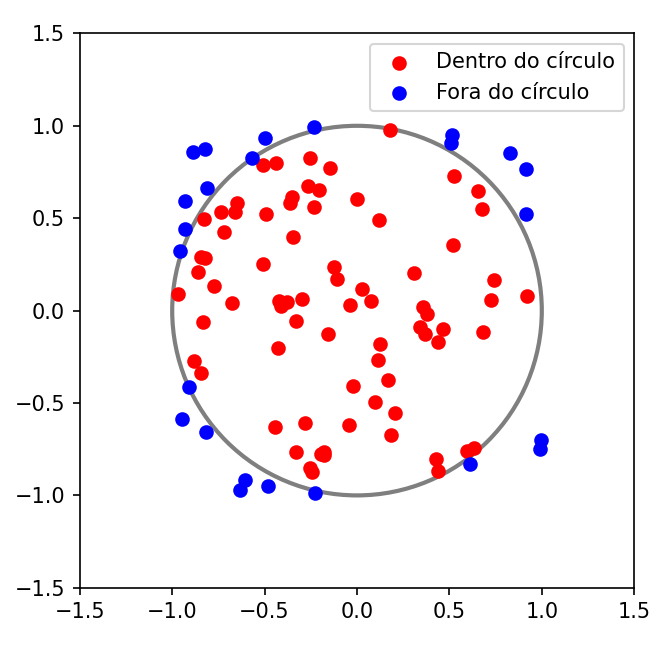
\includegraphics[width=0.7\textwidth]{circulo.png}
  \caption{Estimativa de $\pi$ com 100 pontos}
  \label{fig:circulo}
\end{figure}

\vspace{0.5cm}

Ao usarmos a função $NovaEstimativa(n)$ (com duração de 1min aproximadamente), ela irá utilizar os valores definidos para o número de amostragens, que utilizamos principalmente a variância $\sigma^2 = p(1-p)$ baseada em uma Bernoulli, de $p = \frac{\pi_{estimado}}{4}$. Com os dados mencionados, obtemos que:

\begin{center}

$\sigma_{estimado}^2 = (\frac{3.04}{4} \cdot (1-\frac{3.04}{4})) = 0.1824 $

\end{center}

Assim, obtemos o resultado de $\varepsilon$ ao avaliarmos que: 

\begin{center}

$\frac{4\varepsilon}{\pi_{estimado}} = 0.0005 \implies \varepsilon = 0.000125\pi_{estimado} $

\end{center}

Que torna:

\begin{center}

$\varepsilon = 0.000125 \cdot 3.04 = 0.00038$

\end{center}

Agora, para calcularmos $n$:

\begin{center}

$n = (\frac{z\sigma}{\varepsilon})^2 = (\frac{1.96}{0.00038})^2\cdot0.1824 \approx 4852548 $ 

\end{center}

Assim, precisamos de $4852548$ pontos para termos um $\pi$ com  erro relativo em até $0.05\%$ para tal amostragem.

\end{document}
